%% This is file `elsarticle-template-1-num.tex',
%%
%% Copyright 2009 Elsevier Ltd
%%
%% This file is part of the 'Elsarticle Bundle'.
%% ---------------------------------------------
%%
%% It may be distributed under the conditions of the LaTeX Project Public
%% License, either version 1.2 of this license or (at your option) any
%% later version.  The latest version of this license is in
%%    http://www.latex-project.org/lppl.txt
%% and version 1.2 or later is part of all distributions of LaTeX
%% version 1999/12/01 or later.
%%
%% Template article for Elsevier's document class `elsarticle'
%% with numbered style bibliographic references
%%
%% $Id: elsarticle-template-1-num.tex 149 2009-10-08 05:01:15Z rishi $
%% $URL: http://lenova.river-valley.com/svn/elsbst/trunk/elsarticle-template-1-num.tex $
%%
\documentclass[preprint,12pt]{elsarticle}

%% Use the option review to obtain double line spacing
%% \documentclass[preprint,review,12pt]{elsarticle}

%% Use the options 1p,twocolumn; 3p; 3p,twocolumn; 5p; or 5p,twocolumn
%% for a journal layout:
%% \documentclass[final,1p,times]{elsarticle}
%% \documentclass[final,1p,times,twocolumn]{elsarticle}
%% \documentclass[final,3p,times]{elsarticle}
%% \documentclass[final,3p,times,twocolumn]{elsarticle}
%% \documentclass[final,5p,times]{elsarticle}
%% \documentclass[final,5p,times,twocolumn]{elsarticle}

%% The graphicx package provides the includegraphics command.
\usepackage{graphicx}
%% The amssymb package provides various useful mathematical symbols
\usepackage{amssymb}
%% The amsthm package provides extended theorem environments
%% \usepackage{amsthm}

%% The lineno packages adds line numbers. Start line numbering with
%% \begin{linenumbers}, end it with \end{linenumbers}. Or switch it on
%% for the whole article with \linenumbers after \end{frontmatter}.
\usepackage{lineno}


%% natbib.sty is loaded by default. However, natbib options can be
%% provided with \biboptions{...} command. Following options are
%% valid:

%%   round  -  round parentheses are used (default)
%%   square -  square brackets are used   [option]
%%   curly  -  curly braces are used      {option}
%%   angle  -  angle brackets are used    <option>
%%   semicolon  -  multiple citations separated by semi-colon
%%   colon  - same as semicolon, an earlier confusion
%%   comma  -  separated by comma
%%   numbers-  selects numerical citations
%%   super  -  numerical citations as superscripts
%%   sort   -  sorts multiple citations according to order in ref. list
%%   sort&compress   -  like sort, but also compresses numerical citations
%%   compress - compresses without sorting
%%
%% \biboptions{comma,round}

% \biboptions{}

\journal{Journal Name}

\usepackage[top=1in, bottom=1.5in, left=1in, right=1in]{geometry}
\usepackage[
    %backend=biber, 
    natbib=true,
    style=numeric,
    sorting=none
]{biblatex}
\addbibresource{sample.bib}

\begin{document}


%\begin{frontmatter}

%% Title, authors and addresses

%\title{b~flavored Jets as a Handle for Direct Measurement of ggH production of the Higgs and its subsequent decay to $b\bar{b}$ during Run 3 and Run 4 at the LHC/HL-LHC}

%% use the tnoteref command within \title for footnotes;
%% use the tnotetext command for the associated footnote;
%% use the fnref command within \auth or or \address for footnotes;
%% use the fntext command for the associated footnote;
%% use the corref command within \author for corresponding author footnotes;
%% use the cortext command for the associated footnote;
%% use the ead command for the email address,
%% and the form \ead[url] for the home page:
%%
%% \title{Title\tnoteref{label1}}
%% \tnotetext[label1]{}
 %\author{Prof. Isobel Ojalvo}
 %\ead{iojalvo@princeton.edu}
%% \ead[url]{home page}
%% \fntext[label2]{}
%% \cortext[cor1]{}
%% \address{Address\fnref{label3}}
%% \fntext[label3]{}


%% use optional labels to link authors explicitly to addresses:
%% \author[label1,label2]{<author name>}
%% \address[label1]{<address>}
%% \address[label2]{<address>}

%\author{John Smith}

%\address{California, United States}

%\begin{abstract}
%% Text of abstract
%Suspendisse potenti. Suspendisse quis sem elit, et mattis nisl. Phasellus consequat erat eu velit rhoncus non pharetra neque auctor. Phasellus eu lacus quam. Ut ipsum dolor, euismod aliquam congue sed, lobortis et orci. Mauris eget velit id arcu ultricies auctor in eget dolor. Pellentesque suscipit adipiscing sem, imperdiet laoreet dolor elementum ut. Mauris condimentum est sed velit lacinia placerat. Vestibulum ante ipsum primis in faucibus orci luctus et ultrices posuere cubilia Curae; Nullam diam metus, pharetra vitae euismod sed, placerat ultrices eros. Aliquam tincidunt dapibus venenatis. In interdum tellus nec justo accumsan aliquam. Nulla sit amet massa augue.
%\end{abstract}


%\begin{keyword}
%Science \sep Publication \sep Complicated
%% keywords here, in the form: keyword \sep keyword

%% MSC codes here, in the form: \MSC code \sep code
%% or \MSC[2008] code \sep code (2000 is the default)

%\end{keyword}

%\end{frontmatter}

%%
%% Start line numbering here if you want
%%
%\linenumbers

%% main text


\noindent
\textbf{Acceleration of Track Reconstruction at CMS Using FPGA Co-processors}

\section{Overview}
\label{S:1}
As a member of the CMS experiment~\cite{CMS-JINST}, I propose to continue work developing both
traditional and Machine Learning track based reconstruction on FPGA co-processors.
While acceleration using FPGA co-processors is a new endeavor for my group 
(as well as for the CMS collaboration) I have contributed to and served 
in leadership positions in the CMS collaboration first as the developer of
high speed algorithms for the the Level-1 trigger, put into place in 2015,
then as the convener of the tau trigger development group (2014-2015) 
and later as the convener of the tau physics object group (2015-2018).
Currently, I serve as the US CMS Level-1 Trigger Operations deputy.
I am working with my postdoc Savannah Thais and graduate student Gage DeZoort
on the development of low latency track reconstruction algorithms
that can be run either online (in an upgraded High Level Trigger (HLT)) or offline
(either integrated into future computing facilities or in cloud based services~\cite{Duarte_2019}). 

As a new faculty member at Princeton University, my research focus is 
on the development of optimized algorithms for the CMS trigger system.
We have recently hired a dedicated firmware engineer, Luis Moreno Perez,
who is working with the US CMS APD consortium to develop and design firmware
for trigger processor boards that use Xilinx Virtex 7 and Ultrascale+ 
Field Programmable Gate Arrays (FPGAs) for high speed data processing.
We are working in collaboration with the Princeton computing group led by Peter Elmer,
with David Lange and Bei Wang, on track reconstruction optimization. 
I also serve on the local organizing committee of the 2020 Connecting the Dots 
workshop series which will be hosted at Princeton University. This workshop
series brings together 
experts on track reconstruction and other problems involving pattern recognition 
in sparsely sampled data. While the main focus will be on High Energy Physics (HEP) 
detectors, the Connecting The Dots workshop is intended to be inclusive across other
scientific disciplines wherever similar problems or solutions arise. 

\section{Proposed Research Direction}
The unambiguous identification of an event produced at the 
LHC which contains a clear signature of Dark Matter, or perhaps 
a SuperSymmetric particle would completely change our understanding 
of the physical universe. However, the difficulty surrounding sifting through 
large data sets to identify a tiny fraction of interesting events 
will only grow in the next ten years as data rates are expected to 
increase dramatically while physicists search for increasingly rare 
events and interactions. On the LHC ring, in the ATLAS and CMS detectors 
collisions between particle bunches occur 40 million times per second. 
During LHC Run 2 (2015-2018) each bunch collision resulted in an average of 
75 individual proton-proton interactions. In both ATLAS and CMS, close 
to 150 million channels, as illustrated in Figure~\ref{fig:millionchannels}, need to be read out, 
creating a data rate of terabytes per second \cite{RoadMapComputing, big_data_computing}. This rate must be 
reduced by a factor of 10$^{6}$ within a few microseconds and then 
by a further factor of 100 within a few milliseconds in order to be stored
for later analysis.
\begin{figure*}[htbp]
\centering
     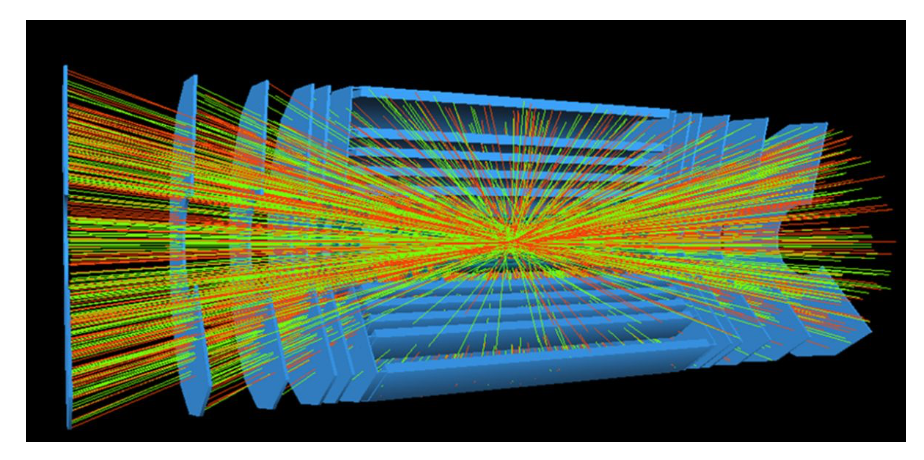
\includegraphics[trim=0 0 0 0,clip,width=0.65\textwidth]{MillionChannels.png}
     \caption{The CMS detector has over 100 million channels. As the number of simultaneous collisions increase from an average of 75 in 2018 to 200 in the 2026 and beyond, 
     reconstruction of charged particle tracks will become an increasingly complex problem.}
     \label{fig:millionchannels}
\end{figure*}

%% 
%% Acceleration Component - streamline, 
%%research plan
%% 1.) visualization exercise
%% 2.) Node features
%% 3.) 
%% 4.) Parallelization on FPGAs
%% Outline problem - Why GNNs
%%copied

Track finding and fitting is one of the most computationally challenging 
problems for event reconstruction in particle physics.
The CMS experiment has 
a specialized tracking system that consists of multiple layers of highly granular 
sensors which are designed to measure both the position and the curvature of the 
charged particle. The many layers and multiple possible paths for each charged 
particle turns the track reconstruction into a highly complex "connecting the dots" 
problem, as illustrated in Fig. 3.
Currently at CMS, track reconstruction relies on the Kalman filter method. 
The filter proceeds iteratively from the seed layer, starting from a coarse estimate of 
the track parameters provided by the seed, and including the
information of the successive detection layers one by one. 
On each layer, i.e. with every new measurement, the track parameters 
are known with a better precision, up to the last point, where they 
include the full tracker information.
The Kalman Filter method is highly tuned for physics performance in today’s LHC 
conditions but the computation time has been shown to scale quadratically or worse with 
detector occupancy\cite{Cerati_2015}. 


Advanced Machine Learning (ML) poses as an exciting solution to the issue of 
algorithm scalability as many ML algorithms are expected to scale linearly %%cite me  
with detector occupancy.
In particular, the Graph Neural Network (GNN) is interesting option
given its ability to learn effective representations of high-dimensional data 
through training and to model complex dynamics through computationally regular 
transformation techniques.
GNNs were first introduced in \cite{4700287}
and has been applied to a growing variety of problems including social networks,
and 3D Shape analysis \cite{zhou2018graph}. They have already been studied for particle for particle tracking
applications in \cite{farrell2018novel} and for the problem
of particle event classification in \cite{martinez2018pileup,qu2019particlenet}.
The graph is constructed so that the nodes are the hits recorded by the detector and the 
edges are connections of the hits between adjacent detector layers that pass a pre-defined
filter which is tuned to be efficient for tracks resulting from high transverse momentum
particles. 

%insert these
%Monte Carlo truth information, which models the helical path of the charged particle through the detector,
%is used for the training. We plan to test the GNN performance on simulated events with 10 tracks,
%100 tracks and 500 tracks. The completion of this project will result in the mapping out of resource
%usage and latency for various ranges of input data and network architectures.
%We have also submitted proposals to both continue the algorithmic
%research into using FPGAs (DOE Office of Science, SciDAC and ASCR, NSF PHY and OAC), and also for testbed
%compute resources (e.g. NSF CC* and/or MRI Track 1) as well as an eventual potential hardware upgrade
%(NSF MRI Track 2) for the CMS experiment. %% Check me
%Node -> single tracker hit
%Directed Edges -> connect hits
%The GNN will link tracker hits by classifying these edges
\begin{figure*}[htbp]
\centering
     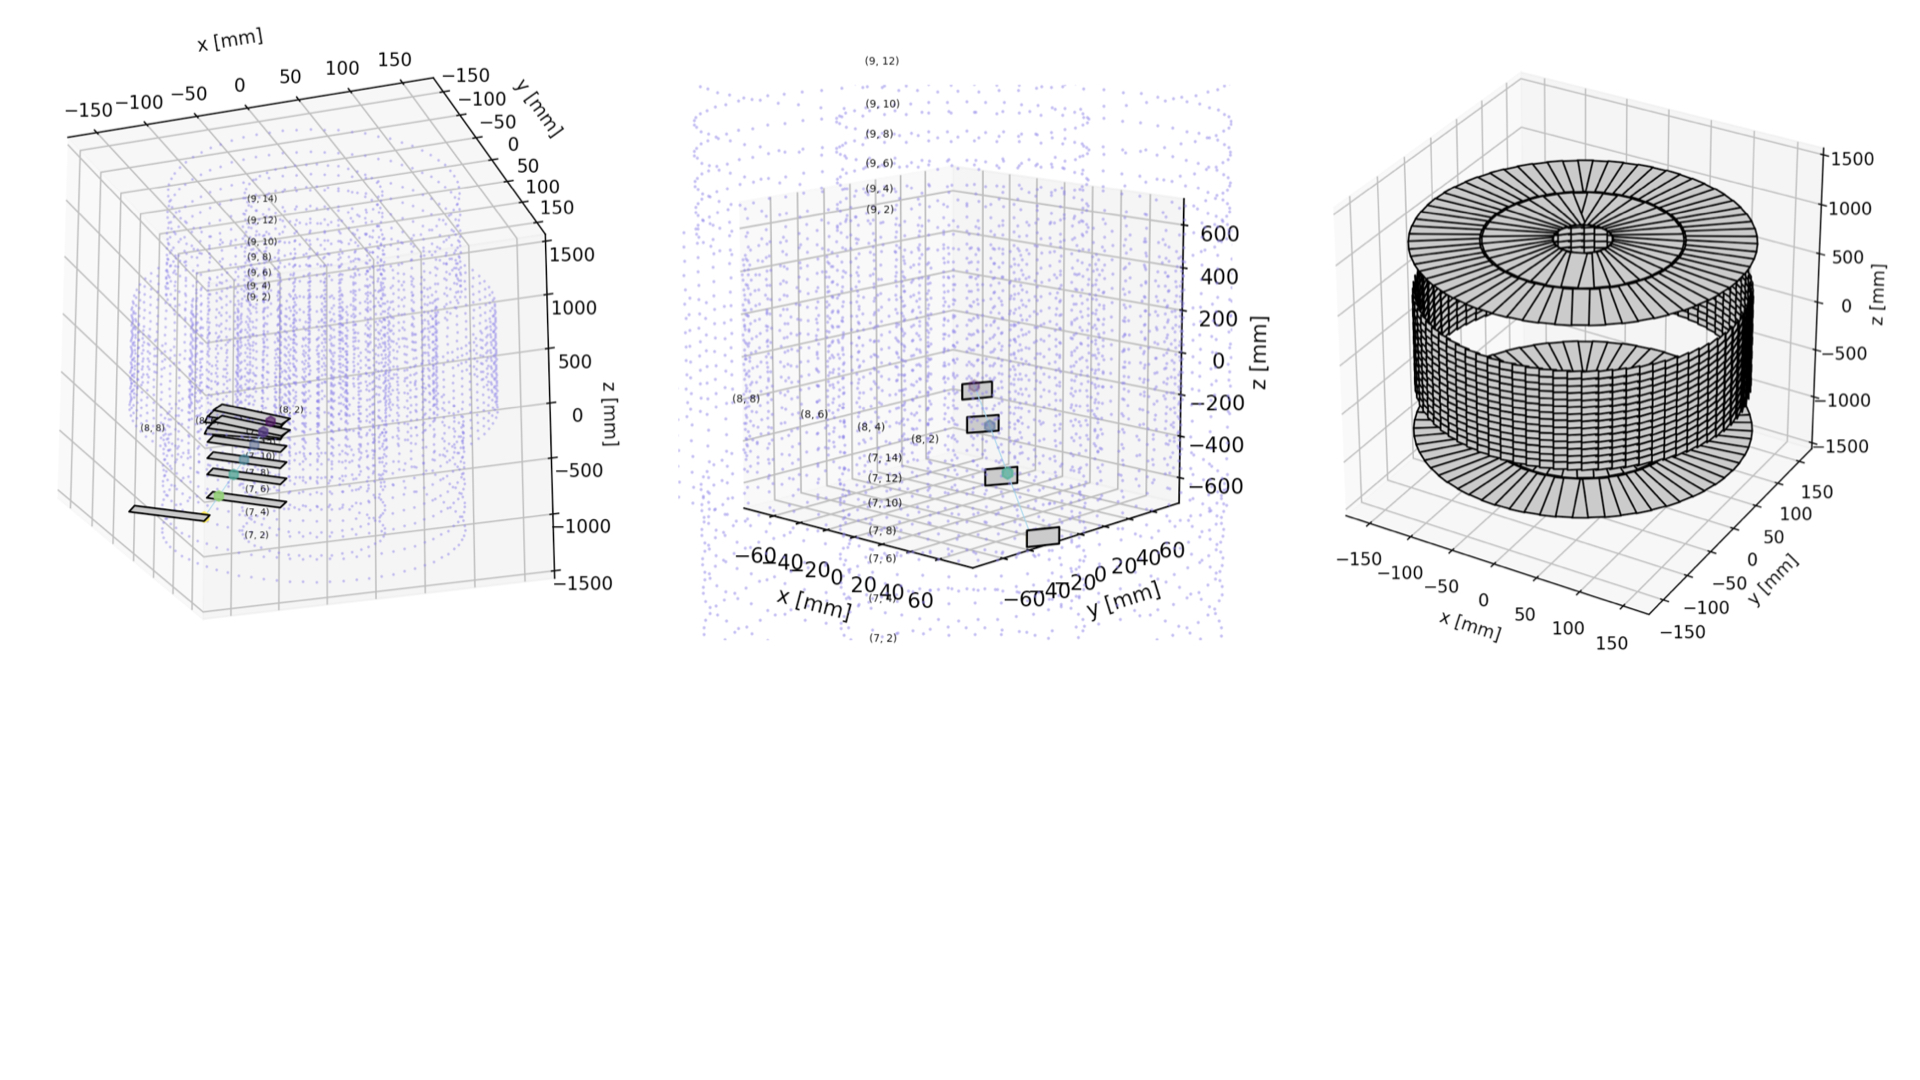
\includegraphics[trim=0 400 0 0,clip,width=0.95\textwidth]{Good_Track_event_display.jpeg}
     \caption{An event display of a high quality track which has at least 3 hits in the pixel layer. Work by postdoc Savannah Thais and graduate student Gage DeZoort.}
     \label{fig:goodtracks}
\end{figure*}

Figure~\ref{fig:goodtracks}, from Princeton postdoc Savannah Thais and graduate student Gage DeZoort,
shows event displays of high quality tracks that are used for training, the tracks are required to
good radial progression (not interactions with the detector) and  have at least 3 hits in the pixel system.
Work done by the Exa.Trkx group \cite{calafiura}
has successfully constructed a GNN architecture which first transforms input node and edge
features into latent representations, a graph module which performs message passing to
update latent features, and an output module which computers edge classification scores.
The encoder uses two fully-connected 2-layer networks for transforming node and edge
features, respectively. The graph module is applied recursively to the latent features.
After N iterations of graph module, the output module takes the last latent features
and uses a 2-layer fully-connected network to produce classification scores for every
edge. All fully-connected layers use a hidden size of 128 and ReLU activation functions,
except the final layer of the output module which uses sigmoid activation.
Studies from this group show that N = 8 graph iterations give the best model
performance.
This indicates great potential for discovering GNN architectures which can scale 
to very large number of edges and that can handle multiple high energy particle 
physics reconstruction tasks. This, in turn, would allow computing centers for 
high energy physics to focus on certain types of acceleration and better determine 
where to spend resources and effort in order to become as efficient as possible.

We have recently started collaborating with the Exa.Trkx group to implement training methods
and to test out GNN on FPGA co-processing.
Our group is also collaborating with Lindsey Gray (CMS, FNAL) on implementation with CMSSW.
We propose to transition the most CPU intensive steps %which ones?
to a highly parallel computing architecture making use of CPUs which have an FPGA co-processor.
The Princeton Research Computing center has recently purchased an Intel Xenon CPU + FPGA co-processor
and similar devices are available at CERN. We are excited to share progress regularly 
in USCMS forums and to collaborate with members of 
both the physics and computer science communities for advancement. 


%GNNs were first introduced in [16] and have been applied to a growing variety of problems including social networks, knowledge graphs, recommender systems, and 3D shape analysis [19, 5]. They were first studied for particle tracking applications in [10] and were also studied for the problem of particle and event classification in [3, 13, 15, 7].

%The graph is constructed so that the nodes are the hits recorded by the detector and theedges are connections of the hits between adjacent detector layers that pass a pre-defined filter that is tuned to be efficient for tracks resulting from high transverse momentum particles. In the input graphs, node features are the three cylindrical coordinates (r, φ, z) and edge features are the difference of the coordinates (∆η, ∆φ). The edge labels are 1 if two hits come from the same track, and 0 otherwise.
%The GNN architecture has three components:
%an encoder which transforms input node and edge features into their latent representations, a graph module which performs message passing to update latent features, and an output module which computes edge classification scores. A diagram of the architecture is shown in figure 1. The encoder uses two fully-connected 2-layer networks for transforming node and edge features, respectively. The initial latent features of the nodes and edges are collectively named H0. The graph module is applied recursively to the latent features. At each iteration i the initial features H0 are concatenated onto the current features Hi. This shortcut connection was empirically found to improve model performance. The graph module also uses two fully-connected 2-layer networks, one which computes updated edge features and one which computes updated node features using aggregated incoming edge features. After N iterations of the graph module, the output module takes the last latent features HN and uses a 2-layer fully-connected network to produce classification scores for every edge. All fully-connected layers use a hidden size of 128 and ReLU activation functions, except the final layer of the output module which uses sigmoid activation. We found that using N = 8 graph iterations gave the best model performance.

%%end copied

%% Relevant expertise

\newpage
%% The Appendices part is started with the command \appendix;
%% appendix sections are then done as normal sections
%% \appendix

%% \section{}
%% \label{}

%% References
%%
%% Following citation commands can be used in the body text:
%% Usage of \cite is as follows:
%%   \cite{key}          ==>>  [#]
%%   \cite[chap. 2]{key} ==>>  [#, chap. 2]
%%   \citet{key}         ==>>  Author [#]

%% References with bibTeX database:

%\bibliographystyle{model1-num-names}

%\bibliography{sample.bib}
\printbibliography

%% Authors are advised to submit their bibtex database files. They are
%% requested to list a bibtex style file in the manuscript if they do
%% not want to use model1-num-names.bst.

%% References without bibTeX database:

% \begin{thebibliography}{00}

%% \bibitem must have the following form:
%%   \bibitem{key}...
%%

% \bibitem{}

% \end{thebibliography}


\end{document}

%%
%% End of file `elsarticle-template-1-num.tex'.
